% Options for packages loaded elsewhere
\PassOptionsToPackage{unicode}{hyperref}
\PassOptionsToPackage{hyphens}{url}
%
\documentclass[
]{book}
\title{Estadísticas Oficiales Institucionales}
\usepackage{etoolbox}
\makeatletter
\providecommand{\subtitle}[1]{% add subtitle to \maketitle
  \apptocmd{\@title}{\par {\large #1 \par}}{}{}
}
\makeatother
\subtitle{Guía Metodológica}
\author{Dirección Nacional de Planeación y Estadística Oficina Nacional de Estadística}
\date{2022-01-06}

\usepackage{amsmath,amssymb}
\usepackage{lmodern}
\usepackage{iftex}
\ifPDFTeX
  \usepackage[T1]{fontenc}
  \usepackage[utf8]{inputenc}
  \usepackage{textcomp} % provide euro and other symbols
\else % if luatex or xetex
  \usepackage{unicode-math}
  \defaultfontfeatures{Scale=MatchLowercase}
  \defaultfontfeatures[\rmfamily]{Ligatures=TeX,Scale=1}
\fi
% Use upquote if available, for straight quotes in verbatim environments
\IfFileExists{upquote.sty}{\usepackage{upquote}}{}
\IfFileExists{microtype.sty}{% use microtype if available
  \usepackage[]{microtype}
  \UseMicrotypeSet[protrusion]{basicmath} % disable protrusion for tt fonts
}{}
\makeatletter
\@ifundefined{KOMAClassName}{% if non-KOMA class
  \IfFileExists{parskip.sty}{%
    \usepackage{parskip}
  }{% else
    \setlength{\parindent}{0pt}
    \setlength{\parskip}{6pt plus 2pt minus 1pt}}
}{% if KOMA class
  \KOMAoptions{parskip=half}}
\makeatother
\usepackage{xcolor}
\IfFileExists{xurl.sty}{\usepackage{xurl}}{} % add URL line breaks if available
\IfFileExists{bookmark.sty}{\usepackage{bookmark}}{\usepackage{hyperref}}
\hypersetup{
  pdftitle={Estadísticas Oficiales Institucionales},
  pdfauthor={Dirección Nacional de Planeación y Estadística   Oficina Nacional de Estadística},
  hidelinks,
  pdfcreator={LaTeX via pandoc}}
\urlstyle{same} % disable monospaced font for URLs
\usepackage{longtable,booktabs,array}
\usepackage{calc} % for calculating minipage widths
% Correct order of tables after \paragraph or \subparagraph
\usepackage{etoolbox}
\makeatletter
\patchcmd\longtable{\par}{\if@noskipsec\mbox{}\fi\par}{}{}
\makeatother
% Allow footnotes in longtable head/foot
\IfFileExists{footnotehyper.sty}{\usepackage{footnotehyper}}{\usepackage{footnote}}
\makesavenoteenv{longtable}
\usepackage{graphicx}
\makeatletter
\def\maxwidth{\ifdim\Gin@nat@width>\linewidth\linewidth\else\Gin@nat@width\fi}
\def\maxheight{\ifdim\Gin@nat@height>\textheight\textheight\else\Gin@nat@height\fi}
\makeatother
% Scale images if necessary, so that they will not overflow the page
% margins by default, and it is still possible to overwrite the defaults
% using explicit options in \includegraphics[width, height, ...]{}
\setkeys{Gin}{width=\maxwidth,height=\maxheight,keepaspectratio}
% Set default figure placement to htbp
\makeatletter
\def\fps@figure{htbp}
\makeatother
\setlength{\emergencystretch}{3em} % prevent overfull lines
\providecommand{\tightlist}{%
  \setlength{\itemsep}{0pt}\setlength{\parskip}{0pt}}
\setcounter{secnumdepth}{5}
\usepackage{booktabs}
\usepackage[left=3cm,right=3cm,top=6cm,bottom=6cm]{geometry}
\ifxetex
  \usepackage{polyglossia}
  \setmainlanguage{spanish}
  % Tabla en lugar de cuadro
  \gappto\captionsspanish{\renewcommand{\tablename}{Tabla}  
          \renewcommand{\listtablename}{Índice de tablas}}
\else
  \usepackage[spanish,es-tabla]{babel}
\fi

\usepackage{float}
\ifLuaTeX
  \usepackage{selnolig}  % disable illegal ligatures
\fi
\usepackage[]{natbib}
\bibliographystyle{apalike}

\begin{document}
\maketitle

{
\setcounter{tocdepth}{1}
\tableofcontents
}
\hypertarget{portada}{%
\chapter*{Portada}\label{portada}}
\addcontentsline{toc}{chapter}{Portada}

\begin{center}
\includegraphics[width=0.75\linewidth,]{imagenes/Portada} \end{center}

\hypertarget{intro}{%
\chapter{\texorpdfstring{\textbf{Introducción}}{Introducción}}\label{intro}}

Las sociedades modernas, a diferenencia de las antepasadas, sufren un exceso de información y sin embargo requieren cada vez más de esta para convivir de manera eficiente. Este fenómeno, no sólo atañe a los individuos sino que cada vez y, con mayor frecuencia, se traslada a sus instituciones.

La gestión de la información a nivel de las entidades públicas ha adquirido un papel protagónico durante los últimos años. Muestra de ello, por ejemplo, loe s la dimensión de \emph{Información y Comunicación} del Modelo Integrado de Planeación y Gestión - MIPG en donde se orienta a las entidades públicas a organizar y administrar de una manera eficiente la información bajo custodia institucional.

La guía que se presenta a continuación es un primer intento a nivel institucional por disponer de un documento que fije las directrices y dé las orientaciones requeridas a nivel de la Universidad para la consolidación, construcción y producción de estadísticas oficiciales. para ello, se propone que este ejercicio debe cumplir, como mínimo, los siguientes pasos metodológicos: \emph{caracterización de usuarios, cumplimiento de requisitos de una estadística, caracterización de registros administrativos, procesamiento de datos, comunicación de resultados y cultura estadística}.

\hypertarget{campo-de-aplicaciuxf3n}{%
\chapter{\texorpdfstring{\textbf{Campo de Aplicación}}{Campo de Aplicación}}\label{campo-de-aplicaciuxf3n}}

Esta guía metodológica aplica para la producción de estadísticas oficiales a nivel estratégico en la Universidad Nacional de Colombia. La misma, en principio, no se recomienda para ser usada en la construcción de indicadores de gestión para cuyo caso existe una guía específica.

Esta guís, junto con la guía para la construcción de \href{https://estadisticaun.github.io/G_Procesos/}{indicadores de proceso}, hacen parte de los aportes metodológicos que ofrece la Universidad en pro del fortalecimiento de la actividad estadística a nivel institucional.

\hypertarget{definiciones}{%
\chapter{\texorpdfstring{\textbf{\emph{Definiciones}}}{Definiciones}}\label{definiciones}}

A continuación, se presentan las definiciones que deben ser tenidas en cuenta a la hora de estudiar e implementar la presente guía metodológica.

\begin{itemize}
\tightlist
\item
  \textbf{Estadísticas}
\end{itemize}

Las estadísticas son cifras de interés social e institucional las cuales se caracterizan, en el ámbito de lo público, principalmente por: ser construidas a partir de información poblacional disponible en registros administrativos y censos o inferida a través de estimaciones provenientes de muestras probabilísticas o no probabilísticas; permitir caracterizar/desagregar temporalmente, temáticamente y geográficamente rasgos de interés de los individuos que conforman las poblaciones o muestras de interés; hacer uso conceptos, estándares y nomenclaturas internacionales, nacionales e institucionales que favorezcan su interpretación y comparación; estar conformadas por cifras agregadas de naturaleza descriptiva derivadas de conteos o de mediciones; representar el presente y el pasado a través de la disposición de series de tiempo; ser susceptibles de ser representadas de manera tabular y gráfica (visualización); estar orientadas y delimitadas por normas; ser fácilmente interpretables y accesibles a través de múltiples mecanismos de disposición y divulgación; ser inclusivas; ser construidas a través de un proceso estadístico y finalmente, a partir de la comparación entre e intra poblaciones de las cifras agregadas, facilitar la creación de indicadores estadísticos.

\begin{itemize}
\tightlist
\item
  \textbf{Estadísticas Oficiales}
\end{itemize}

Las estadísticas oficiales incluyen el subconjunto de estadísticas disponibles a nivel nacional y en cada una de las sedes de la Universidad asociadas a poblaciones de interés para la totalidad de procesos y acciones institucionales. Estas, más que emerger y pertenecer a un proceso particular, son útiles y requeridas por la totalidad de los procesos existentes a nivel institucional. Entre las principales categorías que agrupan las estadísticas oficiales de la Universidad tenemos: información de programas académicos, aspirantes y admitidos, matriculados, graduados, docentes, administrativos, investigación, extensión e innovación, capacidad financiera, etc. Las construcción, disposición y actualización de las estadísticas oficiales de la Universidad Nacional de Colombia, así como la disposición de los lineamientos conceptuales, metodológicos y técnicos requeridos para su gestión, se encuentra a cargo de las áreas de estadística adscritas a las direcciones de planeación y estadística en los niveles nacional y sede. La información estadística oficial de la Universidad, en su mayoría, se encuentra disponible o accesible a través del sitio web institucional de estadísticas oficiales (\url{http://estadisticas.unal.edu.co/home/}).

\begin{itemize}
\tightlist
\item
  \textbf{Indicadores Estadísticos}
\end{itemize}

Los indicadores estadísticos conservan, en términos generales, los mismos atributos que las estadísticas, pero a diferencia de estas, este tipo de mediciones requieren de un trabajo técnico de mayor complejidad que el exigido en las estadísticas. Este tipo de mediciones requieren de fórmulas o de procedimientos metodológicos para efectos del cálculo de la medida de interés y pueden ser de naturaleza simple como las tasas, las razones y las proporciones o complejos como los índices y las escalas.

\begin{itemize}
\tightlist
\item
  \textbf{Indicadores de Gestión}
\end{itemize}

Los indicadores de gestión, a diferencia de las estadísticas y los indicadores estadísticos, se caracterizan porque miden el cumplimiento de una apuesta de futuro (meta) o el rango de desempeño asociado a una acción o conjunto de acciones pertenecientes a una política, proyecto o proceso institucional. Para su construcción y medición se requiere la disposición de líneas de base y, dependiendo del tipo de meta o rango de desempeño a ser monitoreado, pueden ser de diferentes tipos: flujo, acumulación, capacidad, reducción, reducción por periodo, stock. Los elementos conceptuales, metodológicos y técnicos que constituyen los indicadores de gestión o cumplimiento difieren de manera significativa respecto de los constitutivos de las estadísticas y los indicadores estadísticos.

\begin{itemize}
\tightlist
\item
  \textbf{Variable}
\end{itemize}

Es una característica asociada a un ámbito de interés que puede variar y cuya variación adopta diversos posibles valores. Los valores asociados a una variable pueden medirse u observarse de manera directa --variables observables- o indirecta -- variables no observables-.

\begin{itemize}
\tightlist
\item
  \textbf{Variables observables}-
\end{itemize}

Cualquier atributo o característica de fácil definición, medición y consenso dentro de un área, disciplina o teoría científica. Hacen referencia a algo que se sabe que existe y que se puede observar, manipular y medir de manera directa. La edad, el sexo o la profesión de una persona, son ejemplos de variables observables y de interés en el ámbito de la educación o las ciencias de la salud, por ejemplo.

\begin{itemize}
\tightlist
\item
  \textbf{Variables no observables}
  Cualquier entidad o categoría conceptual de difícil definición, medición y consenso dentro de un área, disciplina o teoría científica. También conocidas como variables latentes o constructos, hacen referencia a algo que se sabe que existe pero que no se puede observar, manipular y medir de manera directa --no observables-. La inteligencia, la personalidad, la creatividad, el bienestar individual o social, son algunos ejemplos de constructos de interés académico para disciplinas como la psicología, la economía o la sociología; en contraste, por ejemplo, la satisfacción del usuario, lo es para el ámbito de la gestión administrativa.
\end{itemize}

\hypertarget{referentes-normativos-y-conceptuales}{%
\chapter{\texorpdfstring{\textbf{\emph{Referentes Normativos y Conceptuales}}}{Referentes Normativos y Conceptuales}}\label{referentes-normativos-y-conceptuales}}

La presente guia se basa y tiene en cuenta los siguienets referentes institucionales y normativos en materia de gestión de los datos a nivel institucional.

\begin{enumerate}
\def\labelenumi{\arabic{enumi}.}
\tightlist
\item
  \emph{\href{https://www.dane.gov.co/index.php/sistema-estadistico-nacional-sen}{Sistema Estadístico Nacional}}
\item
  \emph{\href{https://www.funcionpublica.gov.co/web/mipg}{Modelo Integrado de Planeación y Gestión - MIPG}}
\item
  \emph{\href{http://siga.unal.edu.co/images/Modulos/Ova/Caracterizacin-de-usuarios-y-partes-interesadas.pdf}{Caracterización de Usuarios y Partes Interesadas}}
\item
  \emph{\href{https://www.dane.gov.co/files/sen/normatividad/NTC-Proceso-Estadistico-PE-1000-2020.pdf}{Norma Técnica de Calidad del Proceso Estadístico - NTCPE 1000}}
\item
  \emph{\href{https://www.funcionpublica.gov.co/eva/gestornormativo/norma.php?i=49981}{Ley de Protección de Datos - Habeas Data}}
\item
  \emph{\href{https://www.funcionpublica.gov.co/eva/gestornormativo/norma.php?i=56882}{Ley Ley de Transparencia y del Derecho de Acceso a la Información Pública Nacional}}
\item
  \emph{\href{https://www.datos.gov.co/}{Política Nacional de Datos Abiertos}}
\item
  \emph{\href{https://www.sen.gov.co/files/sen/Documento\%20Maestro\%20SETE.pdf}{Sistema de Ética Estadística del DANE - SETE}}
\item
  \emph{\href{https://www.dane.gov.co/index.php/sistema-estadistico-nacional-sen/registros-administrativos/documentacion-registros-administrativos}{Documentación de Registros Administrativos - DANE}}
\item
  \emph{\href{https://www.funcionpublica.gov.co/VisualSIE/faces/javax.faces.resource/docs/Documento_operaciones_estadisticas_y_registros_administrativos.pdf}{Registros Administrativos y Operaciones Estadísticas de la Función Pública}}
\item
  \emph{\href{https://estadisticaun.github.io/L_Conceptual/}{Gestión de la Información Cuantitativa en las Universidades}}
\item
  \emph{\href{https://estadisticaun.github.io/L_procesos/}{Lineamientos para la medición de la gestión por procesos en la Universidad Nacional de Colombia}}
\item
  \emph{\href{https://www.dane.gov.co/files/sen/bp/Codigo_nal_buenas_practicas.pdf}{Código Nacional de Buenas Prácticas del Sistema Estadístico Nacional}}
\item
  \emph{\href{https://geoportal.dane.gov.co/}{Geoportal DANE}}
\end{enumerate}

\hypertarget{proceso-estaduxedstico}{%
\chapter{\texorpdfstring{\textbf{\emph{Proceso Estadístico}}}{Proceso Estadístico}}\label{proceso-estaduxedstico}}

Este componente/capítulo presenta los pasos que se deben cumplir en el ejercicio de producción de estadísticas en la Universidad Nacional de Colombia. Este, en principio, debe cumplir con las siguientes fases o pasos metodológicos: \textbf{\emph{usuarios, requisitos de las estadísticas, características de los registros administrativos, procesamiento de las estadísticas, comunicación de resultados y cultura estadística}}.

\hypertarget{usuarios}{%
\section{Usuarios}\label{usuarios}}

Para garantizar el éxito en el ejercicio de construcción y disposición de las estadísticas oficiales en la Universidad, en primer lugar, se debe garantizar un adecuado conocimiento y acercamiento a los usuarios y/o partes interesadas de cada una de las estadísticas disponibles a nivel institucional.

Para garantizar un adecuado conocimiento de los usuarios y las partes interesadas del proceso de producción de una estadística institucional, en principio y como mínimo, debemos implementar las siguientes acciones institucionales. Para una mayor información sobre el procedimiento de caracterización de los usuarios y partes interesadas, la Universidad dispone de la presentación titulada \href{http://siga.unal.edu.co/images/Modulos/Ova/Caracterizacin-de-usuarios-y-partes-interesadas.pdf}{``Caracterización de Usuarios y Partes Interesadas''} (\citet{siga2021}) en el marco del Sistema Integrado de Gestión Académica, Administrativa y Ambiental - SIGA.

\begin{enumerate}
\def\labelenumi{\arabic{enumi}.}
\tightlist
\item
  \emph{Identificar la población a analizar}
\item
  \emph{Definir el periodo de referencia para el análisis de la información}
\item
  \emph{Identificar fuentes y mecanismos de información}
\item
  \emph{Recopilar y consolidar la información}
\item
  \emph{Actuar, divulgar y publicar la información}
\end{enumerate}

\hypertarget{requisitos}{%
\section{Requisitos}\label{requisitos}}

La estadísticas oficiales de la Universidad Nacional de Colombia deben cumplir las siguientes 14 características.

\begin{itemize}
\tightlist
\item
  \textbf{\emph{Característica 1. Población o muestras}}.
\end{itemize}

La \emph{primera} característica de las estadísticas en el contexto de la universidad pública es que estas se extraen y soportan a partir de información disponible en poblaciones o muestras existentes a nivel institucional.

Las estadísticas asociadas a información de tipo poblacional pueden ser de naturaleza diversa de acuerdo con la forma como son obtenidas o consolidadas. En principio, y salvo contadas excepciones, estas pueden ser de tipo transversal, anidado o longitudinal.

Finalmente, las estadísticas asociadas a información de tipo poblacional son aquellas construidas a partir de muestras. Una muestra está conformada por un subconjunto de individuos de una población, los cuales pueden o no ser seleccionados a través de un mecanismo probabilístico. En las muestras, al igual que en las poblaciones, los individuos comparten características comunes sobre las que se está interesado en obtener estadísticas poblacionales de interés nacional, sectorial o institucional haciendo uso para ello de estimaciones inferidas a partir de los comportamientos observados en los individuos que las conforman. Una muestra probabilística

\begin{itemize}
\tightlist
\item
  \textbf{\emph{Característica 2. Cifras agregadas}}.
\end{itemize}

La \emph{segunda} característica de las estadísticas está relacionada con la capacidad que estas tienen para representar la información de manera resumida o agregada. Las estadísticas no existen sin la disponibilidad de cifras descriptivas agregadas, producto de la actividad de contar o de medir, estas son su esencia. Las estadísticas se interesan por el descubrimiento de regularidades sociales, no es de su interés el estudio del comportamiento de rasgos individuales, aunque se valen de ellos para sus propósitos.

Las medidas agregadas asociadas a las estadísticas son aproximaciones de tipo descriptivo que pueden ser de dos tipos: conteos o mediciones.

\begin{enumerate}
\def\labelenumi{\arabic{enumi}.}
\item
  \emph{Conteos}: estadísticas derivadas de variables cualitativas
  El primer tipo de cifras derivadas del proceso de construcción de estadísticas lo conforman aquellas cuyo resultado es el producto de contar los individuos que conforman una población o muestra, o que al interior de estas comparten ciertos rasgos o atributos de interés.
\item
  \emph{Mediciones}: estadísticas derivadas de variables cuantitativas
  El segundo tipo de cifras asociadas a la construcción de estadísticas lo conforman aquellas que miden ciertos parámetros de interés poblacional asociados al comportamiento de los individuos en una o más variables de interés. Mientras que el primer tipo de cifras asociadas a las estadísticas se centra en contar, este tipo de cifras se centra en medir, por ejemplo, las medidas de tendencia central como el promedio, la mediana o la moda; de posición no central como los cuartiles, deciles, quintiles o percentiles; de dispersión como la varianza, la desviación estándar o el rango; de apuntamiento como la kurtosis, y de simetría o asimetría.
\end{enumerate}

\begin{itemize}
\tightlist
\item
  \textbf{\emph{Característica 3. Desagregaciones (temporales, temáticas y geográficas)}}.
\end{itemize}

La \emph{tercera} característica de las estadísticas es la capacidad de disponer y presentar información de manera desagregada. Las desagregaciones a través de las cuales se representa la información institucional, en el contexto de la universidad pública, son de tres tipos: temporales, geográficas/institucionales y temáticas.

\begin{enumerate}
\def\labelenumi{\arabic{enumi}.}
\item
  \emph{Temporales}: hace referencia a la capacidad de las estadísticas para representar la información desde una perspectiva histórica. Implica la consolidación, el almacenamiento y la disposición de las poblaciones y muestras generadas a lo largo del tiempo. Los años, los semestres y, en una menor medida, los trimestres o meses son las variables comúnmente empleadas para la provisión de estadísticas desde una perspectiva temporal.
\item
  \emph{Geográficas}: los individuos que conforman una muestra o población asociada a la construcción de estadísticas generalmente se encuentran distribuidos espacialmente dentro de un territorio o ubicados jerárquicamente dentro de una estructura organizacional. La capacidad de las estadísticas para representar la información desde una perspectiva geográfica o institucional es una de las características esenciales que favorecen el hacer y la toma de decisiones en el contexto de lo público.
\item
  \emph{Temáticas}: las desagregaciones temáticas son características de los individuos que hacen parte de poblaciones o muestras las cuales trascienden el tiempo y la geografía y, al igual que estas, hacen parte constitutiva de las estadísticas. Por ejemplo, el sexo, el género, la edad, las condiciones socioeconómicas, la presencia de discapacidades, entre otras, hacen parte de los tipos de desagregaciones probables de ser tenidas en cuenta en las universidades para caracterizar las poblaciones humanas que hacen parte de sus comunidades.
\end{enumerate}

\begin{itemize}
\tightlist
\item
  \textbf{\emph{Característica 4. Representación tabular y gráfica}}.
\end{itemize}

La \emph{cuarta} característica de las estadísticas está relacionada con la capacidad que estas tienen para ser representadas de manera gráfica y tabular. La representación gráfica es el rostro de las cifras y es el principal instrumento de comunicación para transmitir el mensaje que deseamos a través de la disposición de las estadísticas en el contexto del Estado y desde luego en sus universidades.

\begin{itemize}
\tightlist
\item
  \textbf{\emph{Característica 5. Comparables}}.
\end{itemize}

La \emph{quinta} característica de las estadísticas oficiales está relacionada con la capacidad de ser comparables a nivel institucional, sectorial, nacional e inticional. Para ello, estas debeb hacer uso de estándares nacionales e internacionales. Así mismo, deben disponer y hacer uso de codificaciones y de nomenclaturas en su proceso de construcción.

Por ejemplo, la División Política y Administrativa del País - DIVIPOLA, es un estándar disponible a nivel de país para la identificación de los departamentos y municipios existentes a lo largo de la geografía nacional.

\begin{itemize}
\tightlist
\item
  \textbf{\emph{Característica 6. Múltiples mecanismos de difusión}}.
\end{itemize}

La \emph{sexta} característica de las estadísticas está relacionada con la estrategia de difusión y comunicación de las cifras disponibles a nivel institucional. Las estadísticas, en principio, podrán y deberán ser divulgadas a través de los siguientes mecanismos de difusión:

\begin{enumerate}
\def\labelenumi{\arabic{enumi}.}
\tightlist
\item
  \emph{Boletines o anuarios estadísticos}:
\item
  \emph{Cubos de información (data cubos)}
\item
  \emph{Dashboards}
\item
  \emph{Presentaciones}
\item
  \emph{Folletos o brochures}
\item
  \emph{Redes sociales}
\end{enumerate}

\begin{itemize}
\tightlist
\item
  \textbf{\emph{Característica 7. Uso intensivo de las TIC}}.
\end{itemize}

La \emph{septimea} característica de las estadísticas está asociada con el uso intensivo que estas deben hacer, en la actualidad, de las TIC para su gestión.

La captura, el almacenamiento, la transformación, la construcción, la visualización y comunicación de cifras estadísticas está mediada por el uso de herramientas de tipo tecnológico. Datos derivados de registros administrativos capturados en sistemas de información; información extraída a partir de consultas a estos sistemas en archivos planos o almacenada en bodegas de datos o data lakes; agregación de datos o transformación de los mismos a través del uso de software como Excel o especializados como R, SAS o Python; entrega de resultados a través de datacubos, dashboards o boletines impresos, en archivos pdf o documentos web; construcción de gráficos estáticos y dinámicos, con altos niveles de diseño y con capacidad de interactuar con los usuarios a través de ambientes web y, finalmente, comunicación de los resultados a través de instrumentos modernos como las redes sociales, como se ha mostrado a lo largo de este documento, hacen parte del lenguaje, la cotidianidad y las competencias actuales requeridas para la gestión de las estadísticas en el escenario de lo público y todos estos requisitos, en mayor medida, tienen que ver con el lenguaje que traen consigo las TIC.

\begin{itemize}
\tightlist
\item
  \textbf{\emph{Característica 8. Incluyentes}}.
\end{itemize}

La \emph{octava} característica de las estadísticas está relacionada con la capacidad que este tipo de cifras tienen, en el ámbito de lo público, para representar a las poblaciones que hacen parte de la sociedad sin discriminaciones por razones de sexo, raza, origen, religión, opinión política, filosofía, etc.

\begin{itemize}
\tightlist
\item
  \textbf{\emph{Característica 9. Legales y éticas}}.
\end{itemize}

La \emph{novena} característica de las estadísticas está relacionada con los aspectos legales y éticos que deben ser tenidos en cuenta al momento de su construcción.

En primer lugar, estas deben tener en cuenta los aspectos legales, como por ejemplo, la \href{https://www.funcionpublica.gov.co/eva/gestornormativo/norma.php?i=49981}{Ley de Protección de Datos Personales} o \textbf{Habeas Data}.

En segundo lugar, estas deben ser construidas de manera ética en todo su proceso. En principio, se recomienda implementar los lienamientos definidos por el Departamento Nacional de Estadística DANE a través del \href{https://www.sen.gov.co/files/sen/Documento\%20Maestro\%20SETE.pdf}{Sistema de Ética - SETE}(\citet{SETE}).

\begin{itemize}
\tightlist
\item
  \textbf{\emph{Característica 10. Públicas y transparentes - abiertas}}.
\end{itemize}

Las estadísticas oficiales, además de ser construidas respetando los marcos jurídicos existentes y los principios éticos emitidos por el ente rector del país (DANE) en materia de construcción y disposición de estadísticas oficiales, deben ser dispuestas de manera abierta y accesible para los usuarios de las mismas.

La \emph{décima} carectarística de las estadísticas está relacionada con el principio de transparencia que debe existir en su proceso de construcción. Para ello, se deben tener en cuenta los lineamientos definidos en el marco de la \href{https://www.funcionpublica.gov.co/eva/gestornormativo/norma.php?i=56882}{Ley de Transparencia y del Derecho de Acceso a la Información Pública Nacional} (Ley 1712 de 2014).

\begin{itemize}
\tightlist
\item
  \textbf{\emph{Característica 11. Metadatos}}.
\end{itemize}

La \emph{onceava} característica de las estadísticas implica la disposición de metadados que faciliten su proceso de interpretación y eviten un mal uso de las mismas. Aunque no existe un marco estandarizado a nivel país para la disposición de metatados, se suigiere su construcción y disposición a nivel interno teniendo en cuenta, por ejemplo, la estructura de \href{http://estadisticas.unal.edu.co/menu-principal/cifras-generales/metadatos/}{metadatos} definida en la \href{http://estadisticas.unal.edu.co/home/}{página de estadística} de la Universidad.

\begin{itemize}
\tightlist
\item
  \textbf{\emph{Característica 12. Proceso estadístico}}.
\end{itemize}

La construcción y disposición de estadísticas institucionales requiere la ejecución sistemática y ordenada de un conjunto de actividades conducentes a la disposición de las cifras institucionales requeridas. La \emph{doceava} característica de las estadísticas está relacionada con la necesaria existencia de un proceso estadístico sostenible que garantice la construcción y disposición de las estadísticas institucionales.

Un proceso estadístico se entiende como un ``conjunto sistemático de actividades encaminadas a la producción de estadísticas que comprende, entre otras, la detección de necesidades, el diseño, la recolección, el procesamiento, el análisis y la difusión''. Este conjunto de actividades se debe acompañar a su vez de unos requisitos de calidad para la generación de estadísticas institucionales. Para que las estadísticas oficiales que producela Universidad sean consideradas oficiales, además de estar incluidas en el Plan Estadístico Nacional, deben haber aprobado la evaluación de la calidad estadística establecida por el Sistema Estadístico Nacional (SEN).

\begin{itemize}
\tightlist
\item
  \textbf{\emph{Característica 13. Líneas de base - nuevas estadísticas}}.
\end{itemize}

La \emph{catorceava} y última característica asociada a las estadísticas está relacionada con la capacidad que estas ofrecen para la construcción y el soporte de nuevas estadísticas y, en especial, de sistemas o indicadores más complejos, así como de indicadores de cumplimiento o gestión institucional.

\hypertarget{registros-administrativos}{%
\section{Registros Administrativos}\label{registros-administrativos}}

El proceso de construcción de estadísticas institucionales, una vez se han identificado los usuarios o partes interesadas, así como los requisistos que estas deben cumplir para ser consideradas como tal, consiste en la caracterisación de los registros administrativos.

De acuerdo con el \href{https://www.dane.gov.co/index.php/sistema-estadistico-nacional-sen/registros-administrativos/documentacion-registros-administrativos}{DANE} (\citet{Registros}) y según el \href{https://www.funcionpublica.gov.co/VisualSIE/faces/javax.faces.resource/docs/Documento_operaciones_estadisticas_y_registros_administrativos.pdf}{Departamento Administrativio de la Función Pública}(\citet{RegistrosDAFP}), \textbf{\emph{un registro administrativo}} se define como el conjunto de datos que contiene la información recogida y conservada por entidades u organizaciones en el cumplimiento de sus funciones o competencias misionales.

Por esta razón, los regisros admnistrativos constituyen una fuente importante para la generación de operaciones estadísticas, por la cantidad de variables que manejan y la información que contienen, pues pueden ser utilizados para investigaciones de diferente naturaleza social o económica.

La caracterización de los registros administrativos que sirven de base para la construcción y disposición de estadísticas institucionales se da a través de la disposición de sus metadatos los cuales, en principio, deben contener los siguientes aspectos:

\begin{enumerate}
\def\labelenumi{\arabic{enumi}.}
\tightlist
\item
  \emph{Nombre del registro administrativo}
\item
  \emph{Instancia responsable}
\item
  \emph{Datos de contacto del o los responsables del registro administrativo}
\item
  \emph{Objetivo del registro administrativo}
\item
  \emph{Marco normativo incluído en el registro administrativo}
\item
  \emph{Unidad de observación}
\item
  \emph{Cobertura geográfica}
\item
  \emph{Conceptos básicos}
\item
  \emph{Uso de nomenclaturas y clasificaciones}
\item
  \emph{variables del registro}
\item
  \emph{Metodología para el acopio de los datos}
\item
  \emph{Instructivos, manuales y/o guías para el desarrollo del registro}
\item
  \emph{Control y calidad del registro}
\item
  \emph{Almacenamiento del registro administrativo}
\item
  \emph{Uso del registro administrativo}
\item
  \emph{Accesibilidad}
\end{enumerate}

\hypertarget{procesamiento}{%
\section{Procesamiento}\label{procesamiento}}

El procesamiento de los registros administrativos con el fin de generar/disponer estadísticas institucionales, es una de las fases más importantes en el ejercicio de construcción de estadísticas. Este, a diferencia de los demás pasos definidos, implica un alto componente técnico y estadístico. En la figura que se presenta a continuación, se ilustran los grandes pasos que deden ser tenidos en cuenta al momento de procesar los datos con el objetivo de generar las estadísticas institucionales.

\begin{figure}
\centering
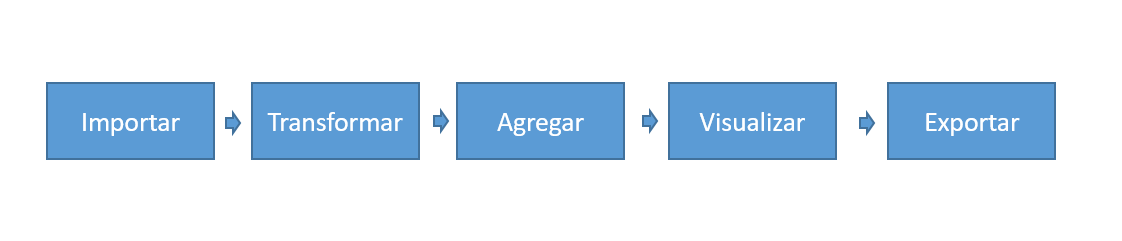
\includegraphics{imagenes/Figura_1.png}
\caption{Figura. Partes del procesamiento de datos}
\end{figure}

Los anteriores pasos implican, en el ámbito de la Universidad, implementar las siguientes acciones.

\begin{enumerate}
\def\labelenumi{\arabic{enumi}.}
\item
  \textbf{\emph{Importar}}: consiste en definir el \textbf{\emph{scrips}} o \textbf{\emph{procedimiento}} de importación de los datos al software que será empleado para la construcción/consolidación de las estadísticas institucionales.
\item
  \textbf{\emph{Transformar}}: consiste en definir el \textbf{\emph{scrips}} o \textbf{\emph{procedimiento}} de transformación y/o depuración de los datos requeridos para la consolidación de los datos institucionales.
\item
  \textbf{\emph{Agregar}}: consiste en definir el \textbf{\emph{scrips}} o \textbf{\emph{procedimiento}} requerido para la agregación de las estadísticas institucionales. Como se ilustró/mencionó en el apartado de requisitos, una de las características centrales de las estadísticas institucionales en su capacidad de presentan cifras agregadas; es decir, consolidados a partir de los individuos que conforman un registro administrativo.
\item
  \textbf{\emph{Visualizar/Tabular}}: consiste en definir el \textbf{\emph{scrips}} o \textbf{\emph{procedimiento}} requerido para la visualización, tabulación y publicación de las cifras oficiales. Los gráficos requeridos para la visualización de la información estadística deben cumplir con las buenas prácticas requeridas para una correcta disposición de los mismos. En contraste, las tablas deben tener la posibilidad de ser dispuestas de manera web.
\item
  \textbf{\emph{Exportar}}: consiste en definir los scrips y/o herramientas tecnológicas requeridas para la disposición/exportación de las estadísticas oficiales. Estas, en la medida de las posibilidades, deben estar dispuestas en plataformas a nivel de \emph{cloud}, en páginas web o en softwares especializados para la disposición de dashboards.
\end{enumerate}

Finalmente, todos los pasos previamente descritos deben contener, de ser posible, los respectivos metadatos que permitan documentar las diferentes acciones implementadas de modo que estos sean fácilmente entendidos por cualquier actor con el dominio técnico requerido.

\hypertarget{comunicaciuxf3n}{%
\section{Comunicación}\label{comunicaciuxf3n}}

La \emph{sexta} característica de las estadísticas está relacionada con la estrategia de difusión y comunicación de las cifras disponibles a nivel institucional. Las estadísticas, en principio, podrán y deberán ser divulgadas a través de los siguientes mecanismos de difusión:

\begin{enumerate}
\def\labelenumi{\arabic{enumi}.}
\tightlist
\item
  \emph{Boletines o anuarios estadísticos}:
\item
  \emph{Cubos de información (data cubos)}
\item
  \emph{Dashboards}
\item
  \emph{Presentaciones}
\item
  \emph{Folletos o brochures}
\item
  \emph{Redes sociales}
\end{enumerate}

\hypertarget{cultura}{%
\section{Cultura}\label{cultura}}

La \emph{septima} característica de las estadísticas está relacionada con el fomento de la cultura estadística a nivel institucional. Para ello, se propone realizar de manera continua un conjunto de acciones, entre las que se sugieren:

\begin{enumerate}
\def\labelenumi{\arabic{enumi}.}
\tightlist
\item
  \emph{Realizar campañas de difusión a través de diversos medios de comunicación}.
\item
  \emph{Socializar los resultados estadísticos en los cuerpos colegiados}.
\item
  \emph{Construir material (físico y multimedia) para facilitar el acceso a la información estadística institucional}.
\item
  \emph{Crear objetos tipo \textbf{Souvenir} para facilitar el acceso a la información estadística institucional}.
\item
  \emph{Fomentar la capacitación y actualización de los funcionarios en matería de gestión estadística}.
\item
  \emph{Participar en eventos de difusión estadística a nivel nacional e internacional}.
\item
  \emph{Patrocinar congresos o eventos institucionales en materia de gestión estadística}.
\item
  \emph{Promocionar la generación de valor de los datos disponibles a nivel institucional a través del fomento a la innovación y la realización de estudios institucionales}.
\end{enumerate}

\hypertarget{gestiuxf3n-del-cambio}{%
\chapter{\texorpdfstring{\textbf{\emph{Gestión del Cambio}}}{Gestión del Cambio}}\label{gestiuxf3n-del-cambio}}

La producción de estadísticas institucionales, a pesar de su historia y trayectoria, está expuesta en la actualidad a un número importante de cambios a nivel conceptual, metodológico, tecnológico, de producción estadística y de gestión de la cultura estadística existente a nivel institucional, que exige la definición de un proceso que le permita adaptarse de manera rápida a los cambios que exige la sociedad.

Por lo anterior, se propone la creación de un procedimiento a nivel de la Universidad Nacional de Colombia que le permita a la gestión estadística institucional adaptarse de manera rápida a los cambios que exige la modernidad.

\hypertarget{referencias}{%
\chapter*{Referencias}\label{referencias}}
\addcontentsline{toc}{chapter}{Referencias}

  \bibliography{book.bib,packages.bib}

\end{document}
